\documentclass[]{../vvsu}

\vvsuyear{2024}

%%%%%%%%%%%%%%%%%%%

\usepackage{graphicx} % для изображений
\usepackage{tabularray} % для таблиц
\usepackage{siunitx} % для обозначений (процент, градус)

% Список путей, где будут искаться изображения и файлы
\graphicspath{{images/}}

% Файл со списком источников
\addbibresource{./references.bib}

%%%%%%%%%%%%%%%%%%%

\begin{document}

% Шапка (опционально, по-умолчанию кафедра ИИТ)
\vvsuhead{МИНОБРНАУКИ РОССИИ\\
ВЛАДИВОСТОКСКИЙ ГОСУДАРСТВЕННЫЙ УНИВЕРСИТЕТ\\
ИНСТИТУТ ИНФОРМАЦИОННЫХ ТЕХНОЛОГИЙ\\
КАФЕДРА ИНФОРМАЦИОННЫХ ТЕХНОЛОГИЙ И СИСТЕМ}

% Название отчета
\title{Магистерская диссертация}
\subtitle{Название темы диссертации} % опционально

% Рекомендация (опционально)
\vvsurecommendation{Заведующий кафедрой\\
канд. экон. наук, доцент}{А.И. Иванов}

% Код работы (опционально)
% GGG,NN - группа
% LL - номер подгруппы
% AAAAAA - номер зачетной книжки
% BBBB - номер приказа
% PP - порядковый номер в приказе
\vvsucode{GGG-NN-LL-AAAAAA.BBBB-с.PP.000.МД}

% Участники работы, может быть любого (разумного) количества
\member{Студент\\ гр. GGG-NN-LL}{А.И. Иванов}
\member{Руководитель\\ Профессор}{А.И. Иванов}
\member{Нормоконтролер\\ канд.физ.-мат.наук, доцент}{А.И. Иванов}
\member{Рецензент\\ канд.физ.-мат.наук, доцент}{А.И. Иванов}

% Вывод титульника
\maketitle

% Аннотация
\begin{addition}{Аннотация}
  Тема ВКР: <<Исследование морских глубин при помощи танцующих роботов>>.

  Автор работы: Студент третьего курса факультета межпланетных дел.

  Руководитель по ВКР: Ведущий научный сотрудник Института бионики.

  Цель ВКР: разработать алгоритм на базе искусственного интеллекта для координации роботов-танцоров под водой и создать на его основе комплексную систему для изучения подводного мира.

  В ходе исследования был проведен анализ проблем подводной навигации и методов синхронизации движений. Для обучения моделей был использован симулированный датасет морских течений. В процессе обучены алгоритмы координации движений, что позволило провести первоначальные тесты на эффективность синхронизации танцев. Параллельно разработана уникальная архитектура искусственного интеллекта, результаты которой были успешно интегрированы в конечную систему. Полученная система успешно прошла тестирование, подтвердив свою эффективность и надежность в экстремальных условиях.

  В ВКР содержится \printtotalpages{}, \printtotalreferences{}, \printtotalfigures{}, \printtotaltables{}.
\end{addition}

% Аннотация на английском
% Аннотация на английском
\begin{addition}{Annotation}
  The topic of the work: "Exploring Quantum Effects in Ice Cream Freezing with Vibrational Sound Waves".

  Author of work: A third-year student from the Department of Galactic Dessert Studies.

  Supervisor: Lead Researcher at the Institute of Advanced Tasteology.

  The purpose of the work: to develop an algorithm based on quantum mechanics to optimize the freezing process of ice cream using vibrational sound waves and to create a comprehensive system for analyzing dessert textures on this basis.

  During the research, an analysis of the subject area was conducted, which included studying the problems of ice cream crystallization and the methods of its enhancement. A dataset was prepared and annotated for training the models. In the process, a classifier and a detector based on spectral analysis were trained, which allowed preliminary tests on the effectiveness of texture recognition. Simultaneously, a proprietary quantum computing architecture was developed, the results of which were compared with the results of the spectral classifiers and detectors. The developed model became the foundation for creating a dessert texture analysis system. Within this system, a specialized component for processing sensory data from taste tests was developed. The final system successfully passed testing, confirming its effectiveness and reliability in dessert innovation.

  The work contains \printtotalpageseng{}, \printtotalreferenceseng{}, \printtotalfigureseng{}, \printtotaltableseng{}.
\end{addition}

% Задание
\begin{addition}{Задание}
  Научно-фантастическая практика по исследованию взаимодействия кофе и гипердрайва включает в себя решение следующих задач:

  \textit{\textbf{Задание 1.}} Анализ альтернативных вселенных:

  \begin{vvsu_list}
    \item описание условий в альтернативных вселенных;
    \item проблемы трансдименсионального перемещения;
    \item постановка задачи оптимизации межвселенского кофе-брейка.
  \end{vvsu_list}

  \textit{\textbf{Задание 2.}} Подготовка коллекции кофе:

  \begin{vvsu_list}
    \item сбор уникальных сортов кофе;
    \item аннотация видео дегустаций и обзоров.
  \end{vvsu_list}

  \textit{\textbf{Задание 3.}} Описание технологий брюинга в условиях нулевой гравитации.

  \textit{\textbf{Задание 4.}} Оформление отчета и документов практики в печатном и электронном виде и представление их на межзвездную конференцию.
\end{addition}

% Содержание
\toc

% Введение
\begin{introduction}
  В современном мире для обнаружения вторжений в космическое пространство широко используются различные автоматические системы, основанные на радарах. Однако у них есть значительные недостатки, включая задержку в обнаружении и трудности с выявлением вторжений на больших расстояниях.

  В случае космического вторжения стандартные радары срабатывают уже тогда, когда объект приблизился слишком близко и представляет реальную угрозу. Например, большие расстояния в космосе не способствуют своевременному обнаружению объектов, когда их еще можно было бы легко отследить. В связи с этим использование систем космического мониторинга более предпочтительно для подобных задач. Однако применение таких систем требует постоянного контроля со стороны операторов.

  Применение систем космического мониторинга исключает ошибки радаров, но ограничивает их до мониторинга человеком. Чтобы уменьшить влияние человеческого фактора и автоматизировать обнаружение вторжений, необходимо использовать системы с применением обученных искусственных интеллектов.

  Цель данной работы - исследовать и разработать алгоритм на базе машинного обучения, который позволит эффективно распознавать неизвестные объекты в космосе. Также данная работа ставит перед собой цель разработать комплексную систему обнаружения космических вторжений, в которой будет применена работа данного алгоритма.
\end{introduction}
\pagebreak

% Глава
\section{Разработка алгоритма обнаружения космических аномалий}

% Под глава
\subsection{Анализ предметной области}

Перед тем как приступить к решению задачи необходимо изучить предметную область, связанную с космическими аномалиями и их обнаружением.

% Под под клава
\subsubsection{Понятия предметной области и статистика}

Согласно Космическому агентству \cite{Space_Agency_Terminology}, космическая аномалия - это неконтролируемое или необычное космическое явление, которое может влиять на работу спутников и других космических аппаратов.

Явление аномалии может включать в себя магнитные бури, радиационные всплески и непредсказуемые изменения в космическом пространстве (таблица \ref{table:space_terms}).

\begin{vvsu_table}{Термины предметной области}
  \label{table:space_terms}
  \begin{tblr}{
    width=1\linewidth,
    colspec={lX},
    hlines, vlines
  }
  Термин   & Значение \\
  Магнитная буря    & Внезапное возмущение магнитного поля Земли, вызванное солнечными вспышками \\
  Радиационный всплеск & Резкое увеличение уровня радиации из-за космических событий, как правило, солнечных вспышек \\
  Космическая изменчивость      & Непредсказуемые изменения в условиях космического пространства \\
  \end{tblr}
\end{vvsu_table}

Для защиты космической техники используются системы космической безопасности, устанавливаемые на спутниках и других аппаратах, которые должны обеспечивать достаточный уровень защиты от космических аномалий.

Состав системы космической безопасности представлен на рисунке \ref{fig:interfaces_scheme}.

\begin{vvsu_figure}{Состав системы космической безопасности}{fig:interfaces_scheme}
  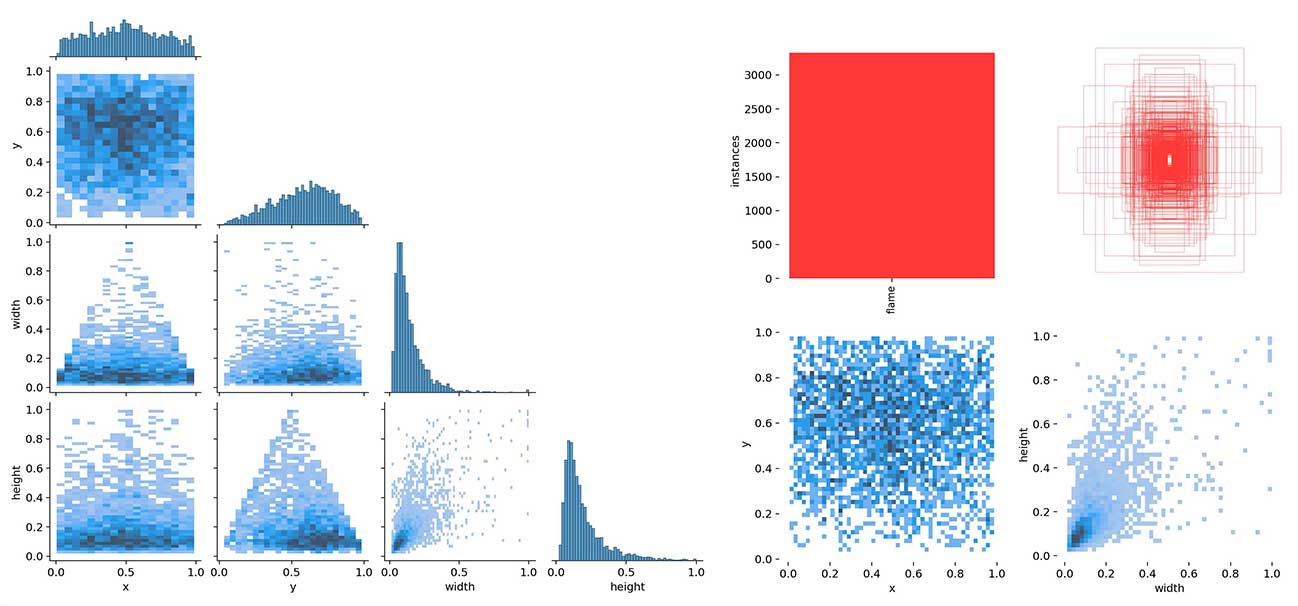
\includegraphics[width=0.8\linewidth]{annotations_information.jpg}
\end{vvsu_figure}

Для предотвращения угроз от космических аномалий используются системы обнаружения - комплекс технических средств и (или) организационных мероприятий, предназначенных для своевременной сигнализации о космических изменениях.

Согласно статистике Космического агентства за 2020 год \cite{Space_Data_2020} произошло $\num{439394}$ космических аномалии, из которых $\qty{70.23}{\percent}$ случаев - из-за солнечных вспышек.

Наиболее частой группой является радиационные всплески ($\qty{69.32}{\percent}$), которые включают в себя:
\begin{vvsu_list}
  \item неосторожное воздействие на радиационные защитные системы;
  \item шалость с радиацией в лабораторных условиях;
  \item прочие причины, связанные с радиационной безопасностью.
\end{vvsu_list}

По данным за первое полугодие 2022 года в космосе произошло $\num{197100}$ космических аномалии. Распределение по типам аномалий показано на рисунке \ref{fig:pie_chart_space_anomalies}.

\begin{vvsu_figure}{Распределение космических аномалий по типам}{fig:pie_chart_space_anomalies}
  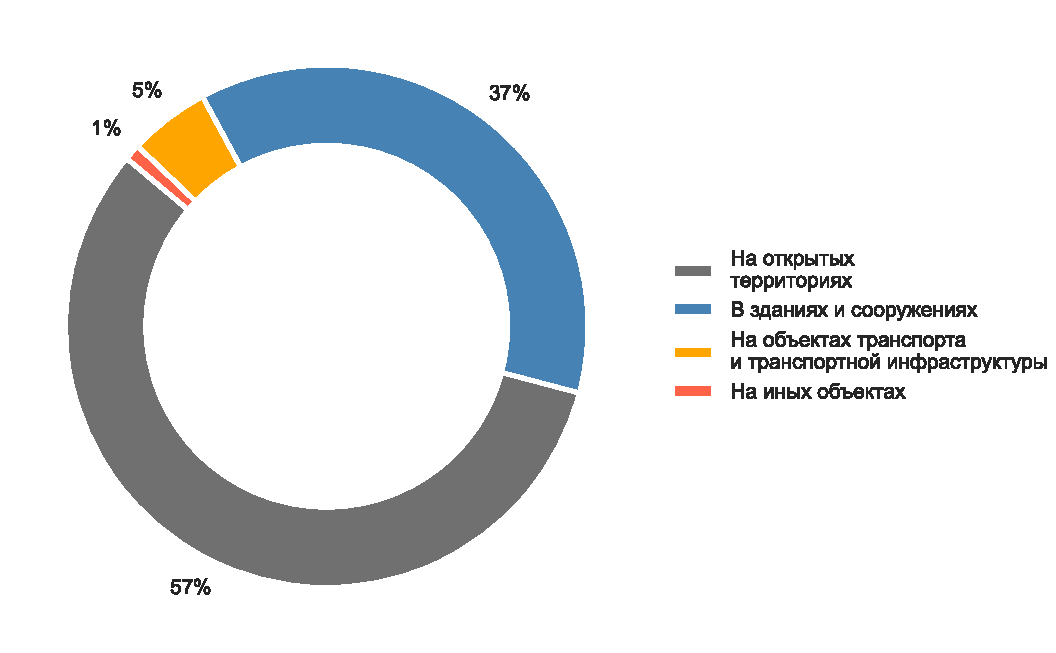
\includegraphics[width=0.9\linewidth]{stats_fire_by_object_groups.pdf}
\end{vvsu_figure}

Наибольшее количество аномалий случается в результате космических изменчивостей ($\qty{57.4}{\percent}$), за ними следуют магнитные бури ($\qty{37.51}{\percent}$).

При сравнении с данными из других космических агентств, наиболее частым местом возникновения космических аномалий являются зоны высокой солнечной активности - $\qty{42.7}{\percent}$ (рисунок \ref{fig:space_anomalies_distribution_chart}).

\begin{vvsu_figure}{Распределение космических аномалий по зонам активности}{fig:space_anomalies_distribution_chart}
  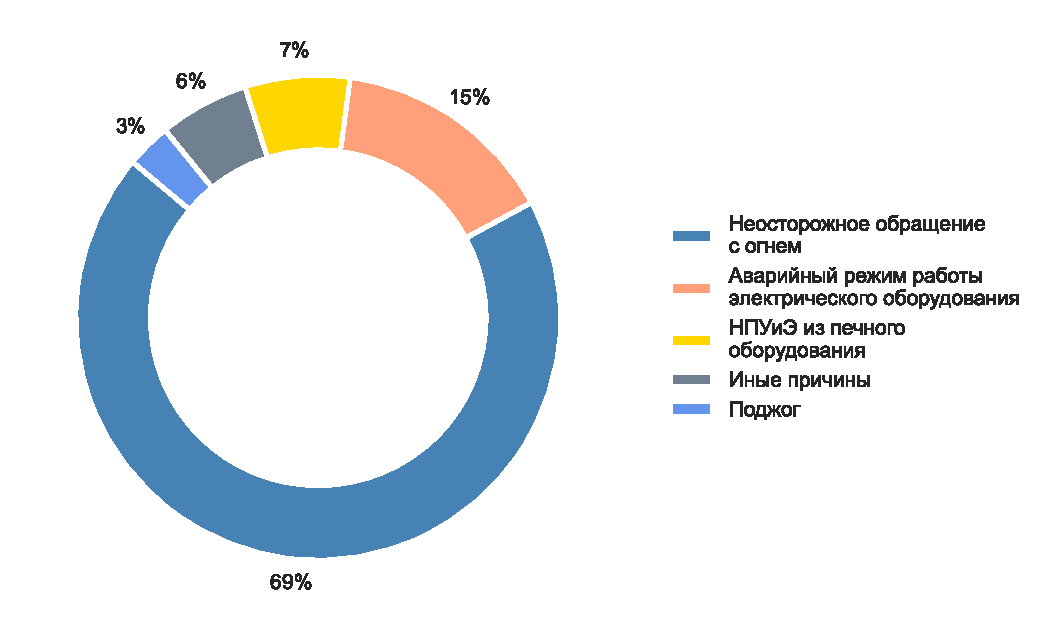
\includegraphics[width=0.9\linewidth]{stats_fire_by_object_reasons.pdf}
\end{vvsu_figure}

Непреднамеренные действия были основной причиной аномалий и возгораний, приведших к потере данных на спутниках и других космических аппаратах.

\subsubsection{Типы космических аномалий и их влияние на космическую аппаратуру}

Для полноценной оценки рисков, связанных с космическими аномалиями, важно понимать основные типы таких явлений и их потенциальное влияние на космическую аппаратуру. Каждый тип аномалии может иметь различные последствия, в зависимости от их интенсивности и продолжительности.

\begin{vvsu_list}
  \item \textbf{Магнитные бури:} Сильные магнитные бури могут вызвать серьезные нарушения в работе электронных систем космических аппаратов. При температурах около $ \qty{1000}{\celsius} $ на поверхности защитных материалов возможно возникновение микротрещин, которые ухудшают защитные свойства.
  \item \textbf{Радиационные всплески:} Во время солнечных всплесков уровень радиации может значительно повыситься, достигая критических значений до $ \qty{500}{\celsius} $ на внешней поверхности спутников, что способствует быстрому старению материалов.
  \item \textbf{Космическая изменчивость:} Непредсказуемые изменения в космическом пространстве могут включать внезапные температурные колебания от $ \qty{-270}{\celsius} $ до $ \qty{150}{\celsius} $, что требует наличия высокоадаптивных тепловых защитных систем.
\end{vvsu_list}

Для каждого типа аномалий разрабатываются специальные меры защиты, включающие использование материалов с повышенной термостойкостью и радиационной устойчивостью, а также системы быстрого реагирования на изменения внешних условий.

\subsection{Расчет влияния радиационных всплесков на орбитальные аппараты}

Радиационные всплески представляют собой кратковременные, но интенсивные увеличения уровня космической радиации, которые могут серьезно повлиять на электронику и материалы космических аппаратов. Важно понимать, как различные уровни радиации воздействуют на космические системы, чтобы обеспечить их надежность и долговечность.

\pagebreak
\section{Оптимизация защитных материалов для космических аппаратов}

Развитие космических технологий требует постоянного улучшения материалов, используемых для защиты космических аппаратов от воздействия экстремальных условий космоса, таких как микрометеориты, космическая радиация и экстремальные температуры. Эффективные защитные материалы способны значительно продлить срок службы аппаратуры и уменьшить затраты на её обслуживание и ремонт.

% Заключение
\clearpage
\begin{conclusion}
  В заключение, разработка межзвездного калькулятора времени путешествий на базе квантовых алгоритмов позволила значительно упростить планирование маршрутов через червоточины. Процесс исследования включал анализ теоретических основ квантовой механики и разработку практических методов их применения. С использованием разработанного алгоритма были успешно проведены испытания в симулированных условиях, что подтвердило его высокую эффективность и точность.

  Внедрение данного калькулятора в практику межзвездных путешествий обеспечивает значительное улучшение точности и безопасности маршрутизации, минимизирует риски потери времени и ресурсов. Помимо технической стороны, проект также способствовал развитию теоретических исследований в области квантовых технологий и стимулировал дальнейшее изучение квантовых эффектов в космических путешествиях.

  Таким образом, данная работа не только решает практическую задачу, но и открывает новые горизонты для научных исследований и технологического прогресса в области космических путешествий.
\end{conclusion}

% Источники
\references

\end{document}